\documentclass[tikz,border=3mm,multi=tikzpicture]{standalone}
\usepackage[utf8]{inputenc}
\usepackage[T1]{fontenc}
\usepackage{helvet}
\renewcommand{\familydefault}{\sfdefault}
\usepackage{tikz}
\usetikzlibrary{arrows.meta,positioning}
\begin{document}

\tikzset{every node/.append style={font=\sffamily\small}}
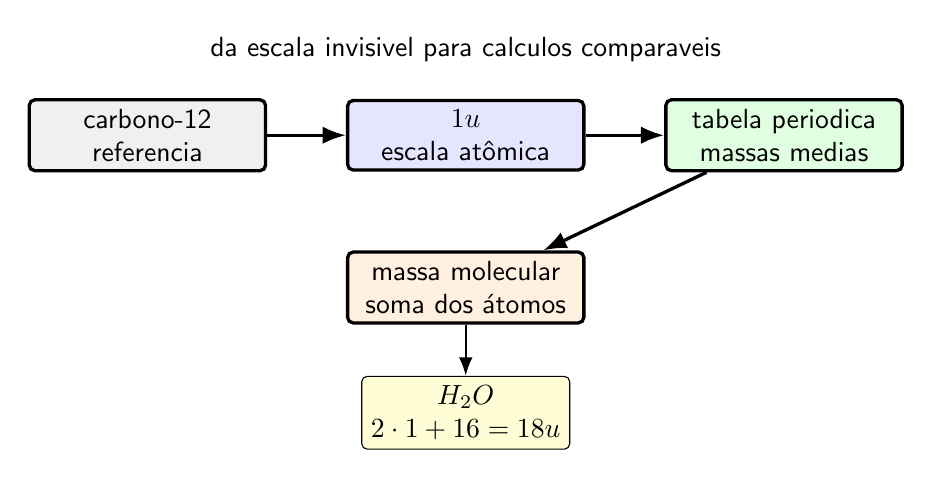
\begin{tikzpicture}[>=Latex,node distance=0.8cm]
  \tikzstyle{box}=[draw,rounded corners=2pt,very thick,minimum width=3cm,minimum height=0.85cm,align=center]
  \node[box,fill=gray!12] (c) {carbono-12\\referencia};
  \node[box,fill=blue!10,right=1cm of c] (u) {$1u$\\escala atômica};
  \node[box,fill=green!12,right=1cm of u] (tab) {tabela periodica\\massas medias};
  \draw[very thick,->] (c) -- (u);
  \draw[very thick,->] (u) -- (tab);
  \node[box,fill=orange!12,below=1cm of u] (mol) {massa molecular\\soma dos átomos};
  \draw[very thick,->] (tab) -- (mol);
  \node[draw,rounded corners=2pt,fill=yellow!16,align=center,below=0.65cm of mol] (ex)
    {$H_2O$\\$2\cdot1 + 16 = 18u$};
  \draw[thick,->] (mol) -- (ex);
  \node[align=center,above=0.35cm of u] {da escala invisivel para calculos comparaveis};
\end{tikzpicture}

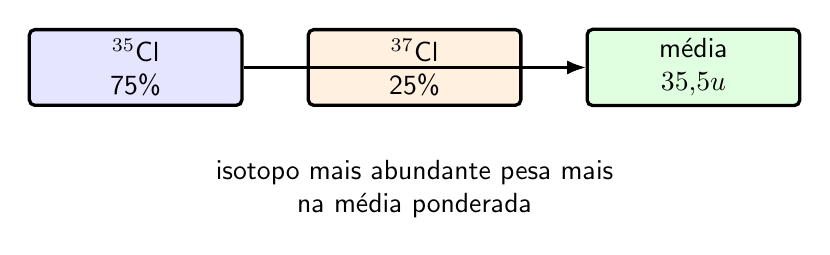
\begin{tikzpicture}[>=Latex,node distance=0.9cm]
  \tikzstyle{box}=[draw,rounded corners=2pt,very thick,minimum width=2.7cm,minimum height=0.85cm,align=center]
  \node[box,fill=blue!10] (cl35) {$^{35}$Cl\\75\%};
  \node[box,fill=orange!12,right=0.8cm of cl35] (cl37) {$^{37}$Cl\\25\%};
  \node[box,fill=green!12,right=0.8cm of cl37] (média) {média\\$35{,}5u$};
  \draw[->,thick] (cl35) -- (média);
  \draw[->,thick] (cl37) -- (média);
  \node[align=center,below=0.55cm of cl37] {isotopo mais abundante pesa mais\\na média ponderada};
\end{tikzpicture}
\end{document}
